\section{Computational Verification and an Image Pilot}
\label{sec:experiments}
We separate exact checks of the algebra from an experiment on learned
visual features. The former can detect implementation errors; the latter
measures reconstruction and class-associated retrieval in one small
setting. Neither substitutes for the other.

\subsection{Exact finite checks}\label{sub:finite-checks}
The executable audit enumerates all $3^{6}=729$ matrices with three
objects, two coordinates, and entries in $\{0,1,2\}$. For each matrix it
checks all eight object subsets and every integer query in the
matrix-bounded product lattice. This gives $41{,}472$ checks of
\cref{eq:adjunction}. It additionally checks object-closure extensivity
and idempotence, preservation of query extents under closure,
join-to-intersection retrieval, and equality with an independently
constructed ordinally scaled binary closure. Empty extents, zero
coordinates, and all-zero matrices are included.

A separate enumeration covers all $3^{4}=81$ two-site, two-coordinate
code arrays and nine queries per array, giving 729 checks of the spatial
inclusion in \cref{prop:spatial-relaxation}. The counterexample with site
codes $(2,0)$ and $(0,2)$ is tested explicitly. All these checks pass.
They verify finite instances and implementation conventions, not the
universal theorems, whose proofs were given above.

\begin{figure}[tbp]
      \centering
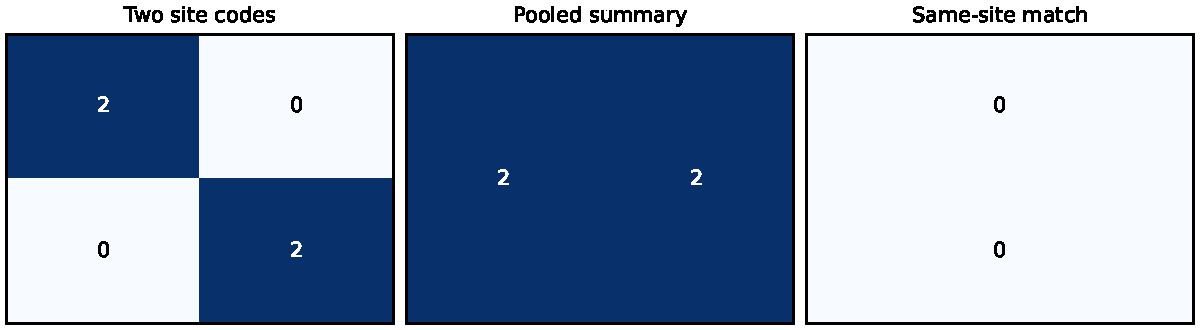
\includegraphics[width=0.85\linewidth]{figures/spatial_example_codexgen.pdf}
      \caption{Constructed example for query $(2,2)$. The pooled summary
satisfies both coordinates, but neither site does. Matrix rows in the
first panel are sites and columns are features. The last panel records
            the two failed same-site tests. These are illustrative codes,
            not activations measured from an image.}
      \label{fig:spatial-example}
\end{figure}

\subsection{Data, training, and reconstruction}
\label{sub:pilot-protocol}
We use the 1,797 grayscale $8\times8$ images supplied by scikit-learn's
\texttt{load\_digits}~\cite{sklearnDigits}. Pixel values are divided by
16. Two stratified splits with random state 2026 yield 1,078 training,
359 calibration, and 360 test images. The split is by image, not by
writer; writer-independent generalization is not tested. The dataset is
the small bundled digits collection, not MNIST or a natural-image corpus.

Each classifier has a padded $3\times3$ convolution from 1 to 16
channels, ReLU, $2\times2$ max pooling, a padded $3\times3$ convolution
from 16 to 32 channels, ReLU, and a linear ten-class head on the flattened
$4\times4\times32$ feature map. We train for 25 epochs with Adam,
learning rate 0.001, batch size 64, and cross-entropy loss. The analysis
sites are the 16 cells after the second ReLU. Their overlapping receptive
fields matter: ``same site'' refers to this feature map, not necessarily
to one small isolated part of the original image.

For each frozen classifier, we train a 32-to-128-to-32 SAE with a linear
encoder, ReLU, and Top-8 selection, using only training-image sites.
The decoder is linear with a bias and unit-length columns, normalized
after every update. Training uses 20 epochs of Adam at learning rate
0.001, batch size 512, and mean squared error, without centering or an
additional sparsity penalty. Classifier and SAE training are repeated
with seeds 17, 29, and 43; all other choices, including the split, remain
fixed. The implementation runs deterministically on CPU with two threads.
No checkpoint or hyperparameter is selected using test performance.

\begin{table}[tbp]
    \centering
    \small
    \caption{Held-out classifier and surrogate diagnostics.}
    \label{tab:reconstruction}
    \begin{tabular}{lrrrrrr}
        \toprule
        Seed & Accuracy & Replaced & $R^{2}_{\rm tr}$ & Site nnz & Image nnz &
        Alive \\
        \midrule
        17   & 96.39    & 95.00    & 0.889            & 8.00     & 15.67     &
        58    \\
        29   & 97.22    & 95.00    & 0.905            & 8.00     & 16.66     &
        53    \\
        43   & 96.39    & 95.56    & 0.925            & 8.00     & 14.95     &
        49    \\
        \bottomrule
    \end{tabular}
\end{table}


In \cref{tab:reconstruction}, ``Accuracy'' and ``Replaced'' are test
classification percentages before and after replacing all analyzed site
activations with SAE reconstructions. The reconstruction statistic is
\begin{equation}\label{eq:reconstruction-statistic}
      R^{2}_{\mathrm{tr}}=1-
      \frac{\sum_{x\in X_{\mathrm{te}}}\sum_{p\in P_{x}}
            \|\widehat h_{x,p}-h_{x,p}\|_{2}^{2}}
      {\sum_{x\in X_{\mathrm{te}}}\sum_{p\in P_{x}}
            \|h_{x,p}-\overline h_{\mathrm{tr}}\|_{2}^{2}},
\end{equation}
where $\overline h_{\mathrm{tr}}$ is the mean over training sites.
It uses a training mean rather than fitting a mean on the test set.
``Site nnz'' and ``Image nnz'' are the mean numbers of positive
coordinates before and after spatial max pooling. ``Alive'' counts
coordinates active anywhere in the training codes.

Reconstruction retains much, but not all, of the classifier's performance.
Only 49--58 of the 128 coordinates are active on training data, so this
pilot is not evidence of an optimized dictionary. Pooling increases the
mean active-coordinate count from 8 to approximately 15--17. This is a
concrete reason to report the object granularity along with sparsity.

\subsection{Queries, calibration, and baselines}
\label{sub:query-protocol}
Each digit supplies a one-versus-rest retrieval task. For each model seed
and digit, we draw five sets of three positive training images without
replacement within a draw; draws can overlap. There are 50 queries per
model and 150 in total. Let $A_{0}$ denote one source set and put
$v=F_{I}(A_{0})$, using max-pooled training codes. Rank coordinates by
$v_{j}/\max(s_{j},10^{-12})$, where $s_{j}$ is the root mean square of
training-image coordinate $j$. Ties are broken by coordinate index.
For the first $b$ ranked coordinates, denoted $T_{b}$, define
\begin{equation}\label{eq:budget-query}
      u_{j}=\begin{cases}
            \alpha v_{j}, & j\in T_{b},    \\
            0,            & j\notin T_{b}.
      \end{cases}
      \qquad
      b\in\{1,4,16,128\},\quad
      \alpha\in\{0.25,0.5,0.75,1\}.
\end{equation}
A coordinate budget can exceed the number of positive coordinates of
$v$; it is an upper bound on query support. This query construction is a
heuristic for selecting sparse evidence, not a lattice-theoretic optimum.

We choose $(b,\alpha)$ separately for each query by maximizing calibration
$F_{1}$, the harmonic mean of precision and recall, with zero returned
when its denominator is zero. Ties follow the displayed increasing
budget and multiplier order. The classifier, SAE, coordinate scales,
and positive source examples all come from training data; calibration
labels select the query parameters. Test images are used only afterwards.

For ranking, the graded satisfaction score is
\begin{equation}\label{eq:graded-score}
      \rho_{u}(x)=\min_{j:u_{j}>0}\frac{u_{x,j}}{u_{j}}.
\end{equation}
For a zero query we use the constant score 1. Thus
$\rho_{u}(x)\geq1$ is exactly pooled query satisfaction. We report average
precision (AP), summing precision over recall increments at distinct
score thresholds. This is a ranking metric; the fixed-cutoff $F_{1}$
measures a different aspect of retrieval. Scaling all positive query
coordinates by a common $\alpha$ leaves their ranking unchanged, but
changes thresholded predictions and can affect the selected budget.

The presence baseline uses the same training-based coordinate ranking
and candidate budgets, replaces each selected positive requirement by
positivity, and selects its budget by calibration $F_{1}$. Its ranking
score is the fraction of these requirements met; its extent requires all
of them. An empty requirement set receives constant score 1. This is an
\emph{amplitude-informed selection with presence-only scoring}, not a
fully binary learning pipeline. It isolates a specific loss of magnitude
information; it does not cover every FCA baseline.

Two cosine baselines compare each test summary with the mean summary of
the same three source images, using either max-pooled SAE codes or the
32-dimensional dense site activations. Zero-norm comparisons receive
score zero. A random-source diagnostic replaces the positive examples
by three arbitrary training images, using the selected graded budget and
multiplier without recalibration. It tests source dependence rather than
serving as an independently optimized competitor. All methods see the
same held-out images. The comparison concerns retrieval from pooled
representations, not the classifier's spatially ordered linear head.

\subsection{Results and their interpretation}
\label{sub:pilot-results}
\begin{table}[tbp]
\centering
\small
\caption{Mean test average precision (percent), 50 queries per seed.}
\label{tab:retrieval}
\begin{tabular}{lrrrr}
\toprule
Method & 17 & 29 & 43 & Mean \\
\midrule
Graded conjunction & 35.65 & 31.80 & 36.37 & 34.60 \\
Presence baseline & 11.83 & 12.47 & 13.29 & 12.53 \\
Sparse-code cosine & 53.96 & 54.70 & 51.48 & 53.38 \\
Dense-code cosine & 66.44 & 67.03 & 68.10 & 67.19 \\
Random sources & 12.83 & 13.12 & 13.02 & 12.99 \\
\bottomrule
\end{tabular}
\end{table}

\begin{table}[tbp]
\centering
\small
\caption{Thresholded retrieval and spatial witnesses on test images.}
\label{tab:spatial}
\begin{tabular}{lrrrrr}
\toprule
Seed & Graded $F_{1}$ & Binary $F_{1}$ & Pooled & Same-site & Mean $\Delta$ \\
\midrule
17 & 0.359 & 0.211 & 4371 & 1347 & 0.667 \\
29 & 0.333 & 0.224 & 4877 & 1776 & 0.610 \\
43 & 0.362 & 0.232 & 4000 & 1232 & 0.720 \\
\bottomrule
\end{tabular}
\end{table}


The graded query improves mean AP over the specified presence baseline
for all three seeds, but both cosine baselines perform better
(\cref{tab:retrieval}). Dense-code cosine gives mean AP 67.19\%, compared
with 34.60\% for graded queries and 12.53\% for presence scoring. The
pilot therefore supports a limited conclusion: amplitudes help within
this conjunctive retrieval design, while these sparse conjunctions are
not the strongest class-retrieval method among those tested.

The test $F_{1}$ scores in \cref{tab:spatial} likewise favor graded over
presence-only satisfaction. Every calibrated graded query has a nonempty
test extent. Budgets 1, 4, and 16 are selected 49, 59, and 42 times,
respectively; budget 128 is never the first maximizing choice. This does
not show that all 128-coordinate candidates perform strictly worse:
with few shared positive coordinates they can coincide with smaller
budgets and lose the specified tie break.

The pooled and same-site totals count query--image matches, so one image
can contribute to many queries. The last column averages
\cref{eq:witness-discrepancy} over the 50 queries for each seed. Its values
show that roughly 61--72\% of pooled matches per query lack a same-site
witness on average. This includes zero discrepancy for queries with one
positive coordinate. The discrepancy is a property of the chosen spatial
quantifiers; it should not be interpreted as an error rate for the model.

\begin{figure}[tbp]
      \centering
      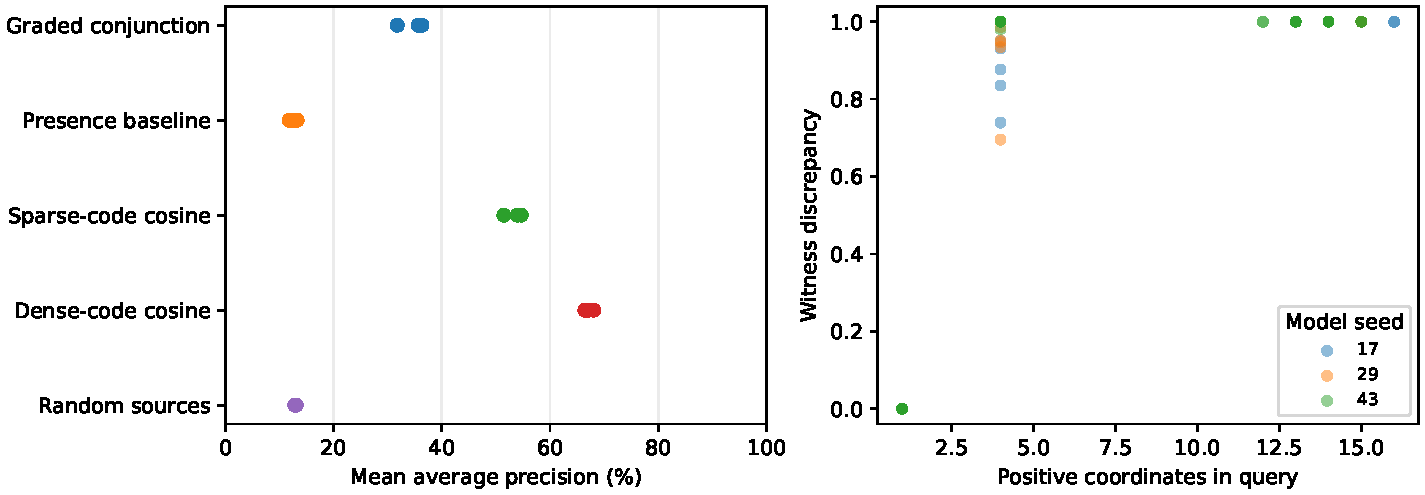
\includegraphics[width=\linewidth]{figures/retrieval_codexgen.pdf}
      \caption{Left: mean test AP for each of the three model seeds. Right:
            witness discrepancy versus actual query support for all 150 graded
queries. Points overlap. These plots describe one fixed image split;
            the seed variation is not a confidence interval over datasets.}
      \label{fig:retrieval}
\end{figure}

\begin{figure}[tbp]
      \centering
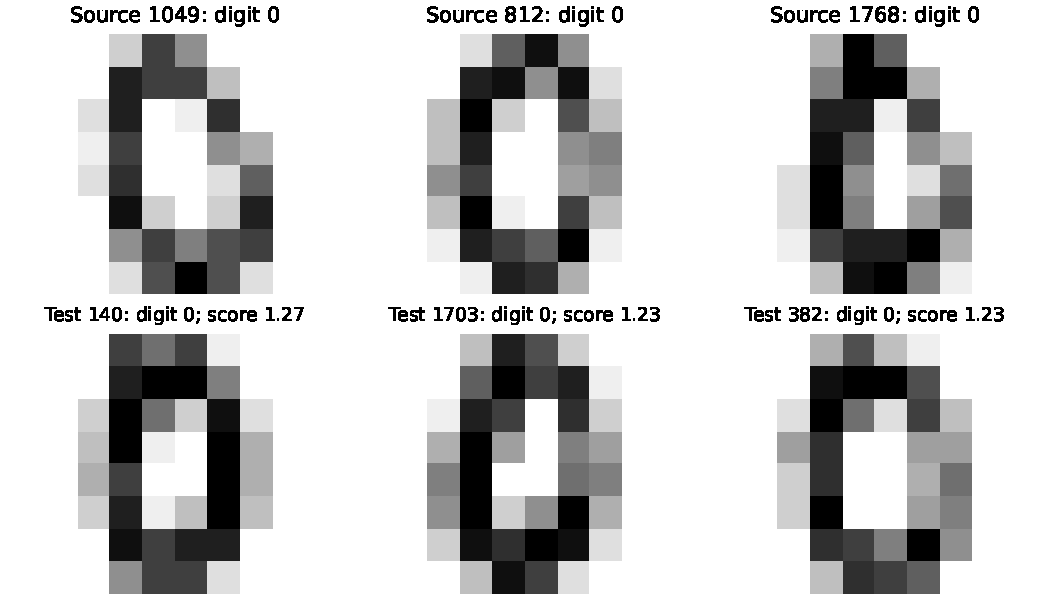
\includegraphics[width=0.75\linewidth]{figures/image_retrieval_codexgen.pdf}
      \caption{An inspectable retrieval example, selected as the first query
in the fixed protocol: seed 17, digit 0, source draw 0. Top: its three
training images. Bottom: the three highest-scoring test images under
            the graded query, with ground-truth digit labels and scores from
\cref{eq:graded-score}. This example is not a semantic annotation of
            the selected latent coordinates.}
      \label{fig:image-retrieval}
\end{figure}

Closure preserves the training extent for all 150 chosen queries, as
required by the theory. We do not replace them by training-closed queries
when evaluating new images: the equality of extents under closure is
relative to the training context and need not survive a change of
object set. The stored queries and scores make this choice explicit.

\subsection{Reproducibility and computational scope}
\label{sub:reproducibility}
The source and reproducibility artifacts are available in the public
Lattice-ML repository~\cite{tsinadzeLatticeML}:
\url{https://github.com/levants/lattice-ml}.
The package separates the context operations, neural models,
experiment runner, algebraic audit, and table generator. The companion
Jupyter notebook reloads cached evidence and checks the reported results.
Saved artifacts include model and SAE weights, site codes, dense
activations, source-image indices, all split indices, query vectors,
test scores, package versions, and SHA-256 hashes. Tables and figures
are generated from the results file rather than edited independently.
The code uses the existing project environment through \texttt{uv}.
Both repositories use the same relative layout: Python modules in
\texttt{src/lattmc/vision}, notebooks in \texttt{notebooks/vision},
and data in \texttt{vision\_tokens}. Within each experiment, datasets,
checkpoints, activation caches, retrieval arrays, and result summaries
are stored separately. Dataset indices and content hashes identify the
exact images and arrays underlying every example.

For $n$ image summaries and a query with $q$ positive coordinates,
retrieval costs $O(nq)$ comparisons. Computing its full closed intent
costs $O(nd)$ in the worst case. Direct same-site testing costs
$O(nPq)$ when each image has $P$ sites. The implementation stores dense
arrays for this small pilot; sparse formats or batched scans are needed
at larger scale. We do not enumerate the full concept lattice, whose
number of concepts can be exponential in the number of objects.
